
% NbTi mass density 
\subsubsection{Mass Density}
The mass density is assumed to be constant and equal to $\rho = 6000~\text{kg/m}^{3}$.

% NbTi specific heat capacity
\subsubsection{Specific Heat Capacity}
Volumetric heat capacity of Nb-Ti is estimated by means of a piece-wise polynomial function which takes into account a linear magnetic dependence below the critical temperature $T_\text{c}$. In order to obtain specific heat capacity in [$\frac{\text{J}}{\text{kg} \cdot \text{K}}$], the function is divided by a constant mass density. The fit parameters are presented in Table \ref{table:nbti_parameters}.

\begin{equation}
    \left\{ \begin{array}{ll}
    Cp_\text{ NbTi}(T, T_\text{c}) = \frac{\text{a}_0 + \text{a}_1\cdot T^{1} + \text{a}_2\cdot T^{2} + \text{a}_3\cdot T^{3}+ \text{a}_4\cdot T^{4}} {\rho_{Nb-Ti}} \\ \\
    T_\text{c}(B) = T_\text{c0}\cdot(1-\frac{B}{B_\text{c20}})^{0.59}
    \end{array} \right.
\end{equation}

\begin{table}[h!]
    \caption{Polynomial parameters} 
    \vspace{-1.em} 
    \fontsize{10}{10}
    \selectfont 
    \renewcommand{\arraystretch}{1.5}
    \begin{center}
    \begin{tabular}{ lccccc }  
    \hline
    & $\text{a}_0$ & $\text{a}_1$ & $\text{a}_2$ & $\text{a}_3$ & $\text{a}_4$ \\
    \hline
    $T \in (0, T_\text{c})$~K & 0 & $64 \cdot B$ & 0 & 49.1 & 0 \\        
    $T \in [T_\text{c}, 28.358)$~K & 0 & 928 & 0 & 16.24 & 0 \\        
    $T \in [28.358, 50.99)$~K & 41383 & -7846.1 & 553.71 & 11.9838 & -0.2177 \\        
    $T \in [50.99, 165.8)$~K & $-1.53\cdot10^{6}$ & 83022 & -716.3 & 2.976 & -0.00482 \\ 
    $T \in [165.8, 496.54)$~K & $1.24\cdot10^{6}$ & 13706 & -51.66 & 0.09296 & $-6.29\cdot10^{-5}$ \\        
    $T \in [496.54, 1000)$~K & $2.45\cdot10^{6}$ & 955.5 & -0.257 & 0 & 0 \\       
    \hline
     \end{tabular} 
    \end{center}  
     \label{table:nbti_parameters} 
 \end{table}
 
 \begin{figure}[h!]
    \centering
    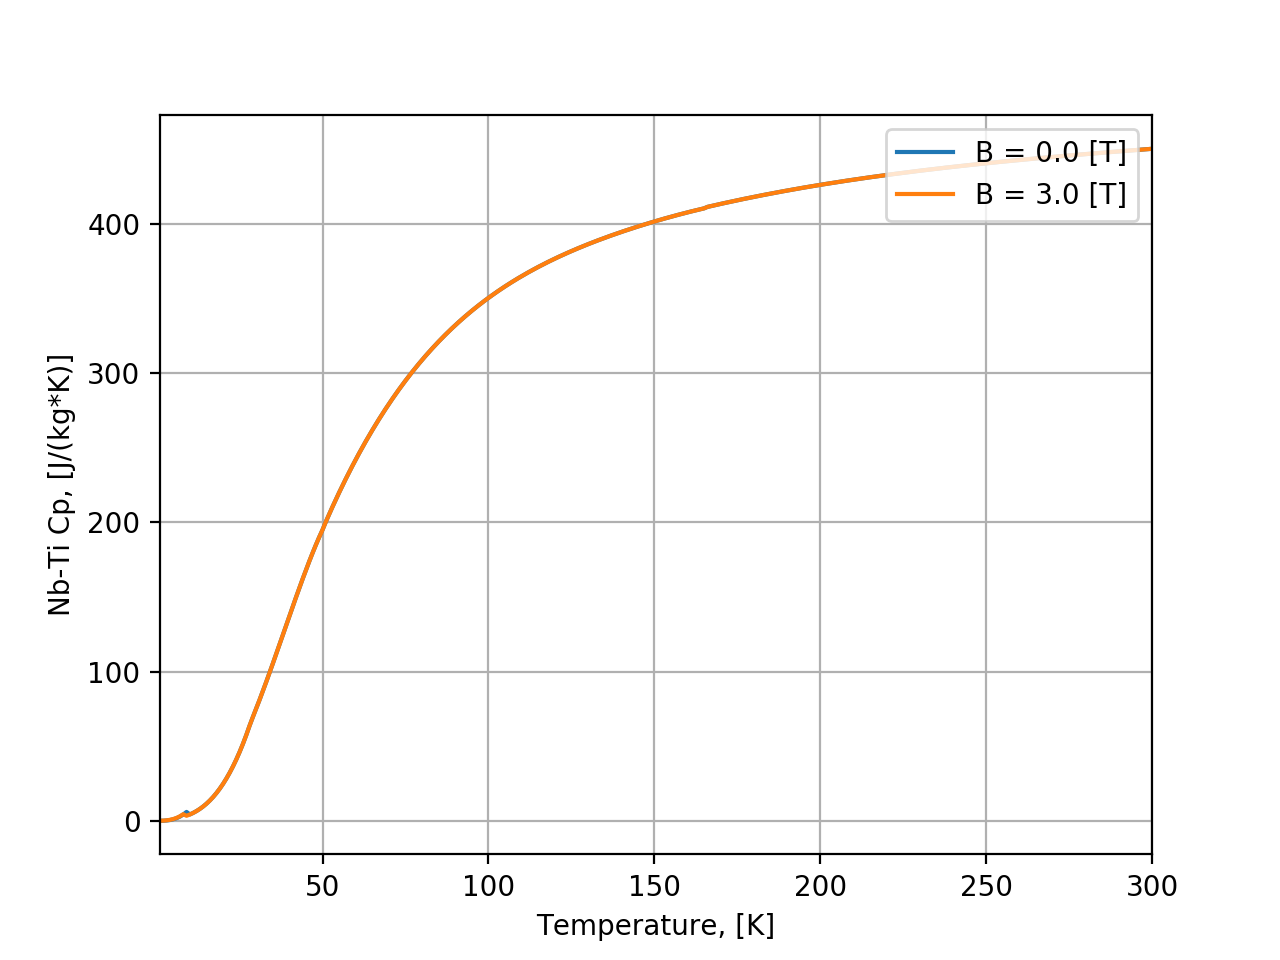
\includegraphics[width=0.49\linewidth]{figures/material_properties/NbTi_Cp_B_Depenedence_plot.png}
    \caption{Nb-Ti specific heat capacity temperature dependence for two values of magnetic field}
    \label{fig:nbti_cp_plot}
\end{figure}
\newpage
